% Number 231
% CVPMA  Units
% Dori/Danica soccer: algebraic version
% JG

% Watermark
\AddToShipoutPicture*{\BackgroundPic}

\addtocounter {ProbNum} {1}

%\begin{floatingfigure}[r]{.4\textwidth}
%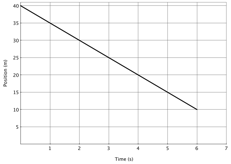
\includegraphics[scale=1]{/Users/jgates/desktop/latex/pics/flipper.png}
%\end{floatingfigure}
 
{\bf \Large{\arabic{ProbNum}}} Dori's running at ${2~\tfrac{m}{s}}$ towards Tower Hill's goal line from 20 meters away when Danica lofts a ball over Dori's head.  The ball hits the ground 3 meters ahead of Dori and rolls towards the goal line at ${4~\tfrac{m}{s}}$.  

\bigskip

It takes 1.5 seconds for Dori to react to the ball; at that point, she begins running faster in order to catch up with the ball before it reaches the goal line.  
%\begin{center} 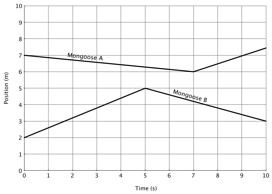
\includegraphics[scale=1]{/Users/jgates/desktop/latex/pics/mongooses.png}
%\end{center}

\bigskip

How fast does she need to run to catch up with the ball before it goes over the goal line? Use algebraic problem-solving.

\vfill

\newpage
